\begin{tikzpicture}[foundation picture]
\node[inner sep=0pt] at (44,80) {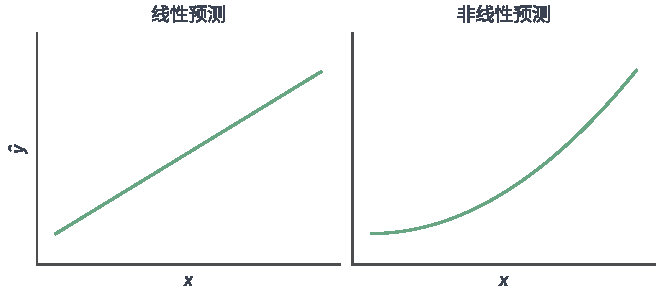
\includegraphics[width=112mm]{figures/02-foundations/01-basics/tikz/models-linear-nonlinear/models-linear-nonlinear.pdf}};
  \foreach \xshift/\title in {0/线性 SVM,56/二次核 SVM}{
    \begin{scope}[xshift=\xshift mm]
      \node[foundation heading] at (16,44) {\title};
      \fill[FigurePaper] (0,0) rectangle (32,32);
      \draw[foundation axis] (1,16)--(35,16) node[right] {$x_1$};
      \draw[foundation axis] (16,1)--(16,35) node[above] {$x_2$};
      \foreach \a in {45,135,225,315}{
        \fill[FigureBlue] ({16+4*cos(\a)},{16+4*sin(\a)}) circle(1);
      }
      \foreach \a in {0,45,90,135,180,225,270,315}{
        \fill[FigureRed]
          ({16+12*cos(\a)-.9},{16+12*sin(\a)-.9})
          rectangle ({16+12*cos(\a)+.9},{16+12*sin(\a)+.9});
      }
    \end{scope}
  }
  \begin{scope}
    \draw[FigureStroke,line width=1.2pt,dashed] (21.5,1)--(21.5,32);
    % 候选分界左侧判为圆点类时，五个方点被错分；空心圈标出这些点。
    \foreach \a in {90,135,180,225,270}{
      \draw[FigureStroke,line width=1.1pt]
        ({16+12*cos(\a)},{16+12*sin(\a)}) circle(2);
    }
  \end{scope}
  \begin{scope}[xshift=56mm]
    \draw[FigureStroke,line width=1.2pt] (16,16) circle(8);
  \end{scope}
\end{tikzpicture}
